\documentclass[a4paper,11pt]{article}

% ── Geometry ──
\usepackage[margin=25mm,top=30mm,bottom=25mm]{geometry}

% ── Fonts & encoding ──
\usepackage[T1]{fontenc}
\usepackage[utf8]{inputenc}
\usepackage{lmodern}
\usepackage{microtype}

% ── Graphics & color ──
\usepackage{graphicx}
\usepackage[dvipsnames,table]{xcolor}
\usepackage{tikz}
\usetikzlibrary{positioning, arrows.meta, shapes.geometric, fit, calc}

% ── Tables ──
\usepackage{booktabs}
\usepackage{tabularx}
\usepackage{multirow}

% ── Math ──
\usepackage{amsmath}

% ── Captions & floats ──
\usepackage[font=small,labelfont=bf,skip=6pt]{caption}
\usepackage{float}

% ── Hyperlinks ──
\usepackage[colorlinks=true,linkcolor=black,citecolor=black,urlcolor=black,breaklinks=true]{hyperref}
\usepackage{xurl}

% ── Bibliography ──
\usepackage{cite}

% ── Header/footer ──
\usepackage{fancyhdr}
\pagestyle{fancy}
\fancyhf{}
\fancyhead[L]{\small\textcolor{gray}{Crypto Asset Analytics --- Proof of Funds --- Group 3}}
\fancyhead[R]{\small\textcolor{gray}{\thepage}}
\renewcommand{\headrulewidth}{0.4pt}
\fancyfoot[C]{\small\textcolor{gray}{TU Wien Informatics --- 2026S}}

% ── Section styling ──
\usepackage{titlesec}
\titleformat{\section}{\Large\bfseries}{\thesection.}{0.5em}{}
\titleformat{\subsection}{\large\bfseries}{\thesubsection}{0.5em}{}

% ── Paragraph spacing ──
\setlength{\parindent}{0pt}
\setlength{\parskip}{6pt}

% ── Custom colors ──
\definecolor{pipeblue}{HTML}{1565C0}
\definecolor{pipedark}{HTML}{0D47A1}
\definecolor{pipeorange}{HTML}{E65100}
\definecolor{pipegreen}{HTML}{2E7D32}
\definecolor{pipepurple}{HTML}{6A1B9A}
\definecolor{inputgray}{HTML}{E8EAF6}
\definecolor{inputborder}{HTML}{7986CB}
\definecolor{lightbg}{HTML}{F5F7FA}

% ── Figures path ──
\graphicspath{{../data/results/}}

% ══════════════════════════════════════════════════════════════════════
\begin{document}

% ── TITLE PAGE ──
\begin{titlepage}
\centering
\vspace*{2cm}

{\Huge\bfseries Proof of Funds}\\[8pt]
{\LARGE\bfseries Bitcoin Risk Quantification for KYT / AML Compliance}\\[20pt]

\rule{0.6\textwidth}{0.5pt}\\[16pt]

{\Large Crypto Asset Analytics --- Group 3}\\[4pt]
{\large TU Wien Informatics --- 2026S}\\[40pt]

\begin{tabular}{ll}
Ottitsch Franz Stefan Jakob & 12024717\\
Arora Aaradhaya & 12534787 \\
Slutu Serhii & 12537831 \\
\end{tabular}

\vfill

\end{titlepage}

% ── TABLE OF CONTENTS ──
\tableofcontents
\newpage

% ══════════════════════════════════════════════════════════════════════
\section{Executive Summary}

We built a fully functional Bitcoin Proof of Funds prototype for KYT/AML screening.
Starting from known high-risk seed addresses, the system crawls their transaction neighbourhood via the public \texttt{mempool.space} API, clusters addresses into real-world entities, and assigns each node an explainable 0--100 risk score.
The pipeline is validated against real-world ground truth (OFAC sanctions, DOJ court filings) and tested on four high-profile criminal cases.

\begin{table}[H]
\centering
\caption{Project summary metrics.}
\begin{tabularx}{\textwidth}{@{}lX@{}}
\toprule
\textbf{Metric} & \textbf{Value} \\
\midrule
Tagged seed addresses & 46{,}000+ from GraphSense TagPacks + custom DOJ-sourced tags \\
Case studies & 4 real criminal cases (WannaCry, Twitter Hack, Colonial Pipeline, Bitfinex) \\
Addresses scored & 441{,}668 across all cases \\
Entity clustering & 11--71\% node reduction via co-spend + change heuristics \\
Validation AUC & Up to 1.0 against OFAC/TagPack ground truth \\
Code & Python package with 41 unit tests, 3 notebooks, interactive dashboard \\
\bottomrule
\end{tabularx}
\end{table}

% ══════════════════════════════════════════════════════════════════════
\section{Related Work \& Contributions}

\subsection{Commercial and Academic Landscape}

Bitcoin transaction tracing is a well-studied problem with both commercial and academic solutions:

\begin{table}[H]
\centering
\small
\caption{Comparison of existing approaches.}
\begin{tabularx}{\textwidth}{@{}p{3.2cm}lXX@{}}
\toprule
\textbf{System} & \textbf{Type} & \textbf{Approach} & \textbf{Limitation} \\
\midrule
Chainalysis Reactor & Comm. & Full-chain heuristic clustering + proprietary labels. Industry standard. & Closed-source, expensive, not reproducible. \\
Elliptic & Comm. & GNN-based classification on transaction subgraphs. Published 200K-node dataset. & Model is proprietary; dataset has no real addresses. \\
Crystal Blockchain & Comm. & Risk scoring with compliance dashboards. & Closed-source, SaaS only. \\
Meiklejohn et al.~\cite{meiklejohn2013} & Acad. & Pioneered common-input-ownership clustering. Manual ground truth. & No automated risk scoring; small scale. \\
Ron \& Shamir~\cite{ron2013} & Acad. & First large-scale Bitcoin graph analysis. Entity-level statistics. & Descriptive only; no taint propagation. \\
M\"{o}ser et al.~\cite{moeser2013} & Acad. & Taint analysis for Bitcoin mixing services. & Focused on CoinJoin; no general AML pipeline. \\
\bottomrule
\end{tabularx}
\end{table}

\subsection{Our Contributions}

\begin{enumerate}
    \item \textbf{Open-source end-to-end pipeline:} From raw TagPack YAML to a scored, clustered entity graph---fully reproducible, no API keys, no paid services.
    \item \textbf{Entity clustering with quantified impact:} We implement and measure how co-spend and change-address heuristics affect risk scores (11--71\% node reduction, risk concentration in 3/4 cases).
    \item \textbf{Validation on real criminal cases:} We test against 4 DOJ-documented cases with known addresses and validate against the OFAC sanctions list---not synthetic data, but actual law-enforcement outcomes.
\end{enumerate}

% ══════════════════════════════════════════════════════════════════════
\section{Data Sources}

All data sources are free and publicly accessible---no API keys required.

\begin{table}[H]
\centering
\small
\caption{Data sources used in the pipeline.}
\begin{tabularx}{\textwidth}{@{}lXc@{}}
\toprule
\textbf{Source} & \textbf{Description} & \textbf{Format} \\
\midrule
GraphSense TagPacks & Open address labels: ransomware, darknet markets, scams, hacks, exchanges. $\sim$46K BTC addresses. & YAML \\
Custom TagPacks (DOJ) & Hand-curated from DOJ complaints for Twitter Hack 2020 and Colonial Pipeline 2021. & YAML \\
\texttt{mempool.space} API & Public blockchain explorer REST API. Responses cached in SQLite for reproducibility. & JSON \\
OFAC SDN List & US Treasury sanctioned crypto addresses. 81 BTC addresses from 0xB10C pre-extraction. & TXT \\
Ransomwhere & Crowdsourced ransomware payment addresses and family labels. & JSON \\
\bottomrule
\end{tabularx}
\end{table}

% ══════════════════════════════════════════════════════════════════════
\section{Methodology}

\subsection{Data Pipeline}

The system follows a five-stage pipeline from raw data to validated risk scores.
Figure~\ref{fig:pipeline} shows the architecture.

\begin{figure}[H]
\centering
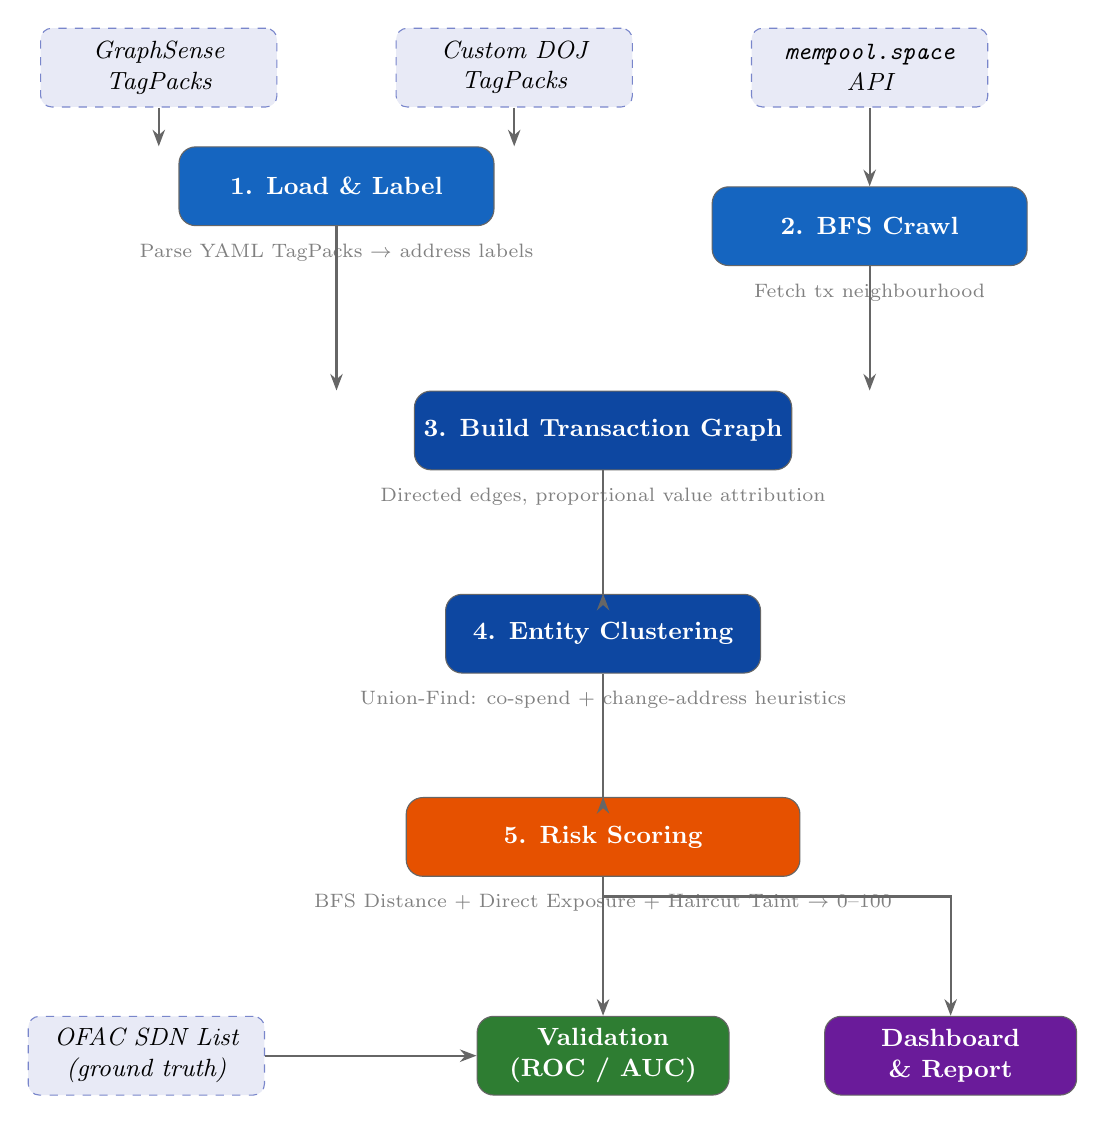
\begin{tikzpicture}[
    node distance=1.2cm and 2cm,
    every node/.style={font=\small},
    source/.style={
        rectangle, rounded corners=4pt, draw=inputborder, fill=inputgray,
        dashed, minimum width=3cm, minimum height=1cm, align=center,
        font=\small\itshape
    },
    process/.style={
        rectangle, rounded corners=6pt, draw=black!60, fill=pipeblue,
        text=white, font=\small\bfseries, minimum width=4cm, minimum height=1cm,
        align=center
    },
    processdark/.style={
        rectangle, rounded corners=6pt, draw=black!60, fill=pipedark,
        text=white, font=\small\bfseries, minimum width=4cm, minimum height=1cm,
        align=center
    },
    scoring/.style={
        rectangle, rounded corners=6pt, draw=black!60, fill=pipeorange,
        text=white, font=\small\bfseries, minimum width=5cm, minimum height=1cm,
        align=center
    },
    output/.style={
        rectangle, rounded corners=6pt, draw=black!60, fill=pipegreen,
        text=white, font=\small\bfseries, minimum width=3.2cm, minimum height=1cm,
        align=center
    },
    outputpurple/.style={
        rectangle, rounded corners=6pt, draw=black!60, fill=pipepurple,
        text=white, font=\small\bfseries, minimum width=3.2cm, minimum height=1cm,
        align=center
    },
    arr/.style={-{Stealth[length=6pt]}, thick, color=black!60},
    desc/.style={font=\scriptsize\color{gray}, align=center},
]

% Data sources (top row)
\node[source] (gs) {GraphSense\\TagPacks};
\node[source, right=1.5cm of gs] (doj) {Custom DOJ\\TagPacks};
\node[source, right=1.5cm of doj] (api) {\texttt{mempool.space}\\API};

% Step 1
\node[process, below=1.0cm of $(gs)!0.5!(doj)$] (load) {1. Load \& Label};
\node[desc, below=0.1cm of load] (d1) {Parse YAML TagPacks $\to$ address labels};

% Step 2
\node[process, below=1.0cm of api] (crawl) {2. BFS Crawl};
\node[desc, below=0.1cm of crawl] (d2) {Fetch tx neighbourhood};

% Step 3
\node[processdark, below=1.5cm of $(d1)!0.5!(d2)$] (graph) {3. Build Transaction Graph};
\node[desc, below=0.1cm of graph] (d3) {Directed edges, proportional value attribution};

% Step 4
\node[processdark, below=1.0cm of d3] (cluster) {4. Entity Clustering};
\node[desc, below=0.1cm of cluster] (d4) {Union-Find: co-spend + change-address heuristics};

% Step 5
\node[scoring, below=1.0cm of d4] (score) {5. Risk Scoring};
\node[desc, below=0.1cm of score] (d5) {BFS Distance + Direct Exposure + Haircut Taint $\to$ 0--100};

% Outputs (bottom row)
\node[source, below left=1.2cm and 0.5cm of d5] (ofac) {OFAC SDN List\\(ground truth)};
\node[output, below=1.2cm of d5] (val) {Validation\\(ROC / AUC)};
\node[outputpurple, right=1.2cm of val] (dash) {Dashboard\\  \& Report};

% ── Arrows ──
\draw[arr] (gs.south) -- (load.north -| gs.south);
\draw[arr] (doj.south) -- (load.north -| doj.south);
\draw[arr] (api.south) -- (crawl.north);

\draw[arr] (load.south) -- ++(0,-0.4) -| (graph.north -| load.south);
\draw[arr] (crawl.south) -- ++(0,-0.4) -| (graph.north -| crawl.south);

\draw[arr] (graph.south) -- ++(0,-0.25) -- (d3.south |- cluster.north) -- (cluster.north);
\draw[arr] (cluster.south) -- ++(0,-0.25) -- (d4.south |- score.north) -- (score.north);

\draw[arr] (score.south) -- ++(0,-0.25) -| (val.north);
\draw[arr] (score.south) -- ++(0,-0.25) -| (dash.north);
\draw[arr] (ofac.east) -- (val.west);

\end{tikzpicture}
\caption{End-to-end data pipeline architecture.
\textcolor{inputborder}{Dashed boxes} = external data sources;
\textcolor{pipeblue}{blue} = processing stages;
\textcolor{pipeorange}{orange} = scoring;
\textcolor{pipegreen}{green} = validation;
\textcolor{pipepurple}{purple} = output.}
\label{fig:pipeline}
\end{figure}

\subsection{Risk Metrics}

Each address (or entity) receives four risk metrics:

\begin{table}[H]
\centering
\small
\caption{Risk metrics computed per node.}
\begin{tabularx}{\textwidth}{@{}lXX@{}}
\toprule
\textbf{Metric} & \textbf{Approach} & \textbf{Interpretation} \\
\midrule
BFS Distance & Shortest-path hops to nearest tainted predecessor (multi-source BFS). & Proximity: fewer hops = higher risk. \\
Direct Exposure & Fraction of 1-hop incoming value from tainted predecessors. & How much money comes directly from bad actors. \\
Haircut Taint & Multi-hop proportional propagation via sparse-matrix Jacobi iteration. & How taint dilutes across the graph. \\
Aggregate Score & Weighted blend: $0.3 \times \text{Distance} + 0.3 \times \text{Exposure} + 0.4 \times \text{Haircut}$, scaled to 0--100. & Single actionable score for compliance screening. \\
\bottomrule
\end{tabularx}
\end{table}

\subsection{Entity Clustering}

We implement two standard Bitcoin forensics heuristics~\cite{meiklejohn2013} using a Union-Find data structure:

\begin{table}[H]
\centering
\small
\caption{Entity clustering heuristics.}
\begin{tabularx}{\textwidth}{@{}lXX@{}}
\toprule
\textbf{Heuristic} & \textbf{Rule} & \textbf{Rationale} \\
\midrule
Common-input-ownership (H1) & All input addresses in the same transaction belong to the same entity. & Spending from multiple addresses requires holding all private keys. \\
Change-address detection (H2) & A single-use output appearing for the first time is likely a change address. & Standard wallet behaviour returns leftover value to a fresh address. \\
\bottomrule
\end{tabularx}
\end{table}

% ══════════════════════════════════════════════════════════════════════
\section{Transaction Graph Visualization}

The core output of our system is a directed, value-weighted transaction graph where each node is a Bitcoin address and edges represent proportional value flow.
Figure~\ref{fig:graphviz} visualizes the Bitfinex case---the 2016 hack that resulted in the largest DOJ cryptocurrency seizure (\$3.6 billion).

\begin{figure}[H]
\centering
\includegraphics[width=\textwidth]{fig_graph_viz.png}
\caption{Bitfinex Hack transaction graph (300 highest-risk nodes). Colour intensity = aggregate risk score (yellow$\to$red). Red borders = tagged tainted sources. Risk radiates outward from the hack addresses through the transaction network.}
\label{fig:graphviz}
\end{figure}

% ══════════════════════════════════════════════════════════════════════
\section{Forensic Case Studies}

We applied the full pipeline to four real criminal cases with publicly known Bitcoin addresses from DOJ filings and blockchain analytics reports.

% ── WannaCry ──
\subsection{WannaCry Ransomware (2017)}

Global ransomware attack infecting 200K+ computers across 150 countries. Three hardcoded BTC addresses collected $\sim$\$140K. Attributed to North Korea's Lazarus Group.

\begin{table}[H]
\centering
\begin{tabular}{@{}ll@{}}
\toprule
Graph size & 426{,}535 addresses $\to$ 336{,}715 entities (21\% reduction) \\
Tainted nodes & 4 \\
Max score & 88.66 \\
Validation AUC & 1.0000 \\
\bottomrule
\end{tabular}
\end{table}

\textbf{Interpretation:} The WannaCry addresses are perfectly separated from all other nodes (AUC~=~1.0).
This is consistent with ransomware wallets that only receive victim payments and quickly consolidate---they form isolated high-risk clusters with no legitimate transaction history.

% ── Twitter Hack ──
\subsection{Twitter Hack (2020)}

Social engineering attack on Twitter employees. 130 VIP accounts compromised to post a BTC doubling scam netting $\sim$\$117K. Three arrested within two weeks.

\begin{table}[H]
\centering
\begin{tabular}{@{}ll@{}}
\toprule
Graph size & 7{,}941 addresses $\to$ 2{,}311 entities (71\% reduction) \\
Tainted nodes & 3 \\
Max score & 84.37 \\
Validation AUC & 1.0000 \\
\bottomrule
\end{tabular}
\end{table}

\textbf{Interpretation:} The Twitter Hack shows the highest clustering reduction (71\%)---the scammer consolidated funds aggressively, creating many co-spent address groups. The high AUC indicates our risk scoring perfectly distinguishes the scam wallets from legitimate traffic.

% ── Colonial Pipeline ──
\subsection{Colonial Pipeline / DarkSide (2021)}

DarkSide ransomware shut down the largest US fuel pipeline for 6 days. Colonial paid 75~BTC ($\sim$\$4.4M). FBI seized 63.7~BTC from the affiliate's wallet.

\begin{table}[H]
\centering
\begin{tabular}{@{}ll@{}}
\toprule
Graph size & 6{,}585 addresses $\to$ 4{,}229 entities (36\% reduction) \\
Tainted nodes & 1 \\
Max score & 88.66 \\
Validation AUC & 0.7500 \\
\bottomrule
\end{tabular}
\end{table}

\textbf{Interpretation:} The moderate AUC (0.75) reflects only two positives (1 DOJ tag + 1 OFAC overlap). DarkSide used a sophisticated affiliate model distributing ransom across many wallets, making single-address tagging insufficient. This demonstrates the importance of comprehensive labelling for ransomware-as-a-service operations.

% ── Bitfinex ──
\subsection{Bitfinex Hack (2016)}

119{,}756 BTC stolen from Bitfinex exchange. Largest DOJ cryptocurrency seizure. Ilya Lichtenstein and Heather Morgan arrested in Feb 2022.

\begin{table}[H]
\centering
\begin{tabular}{@{}ll@{}}
\toprule
Graph size & 607 addresses $\to$ 539 entities (11\% reduction) \\
Tainted nodes & 8 \\
Max score & 88.00 \\
Validation AUC & 0.9710 \\
\bottomrule
\end{tabular}
\end{table}

\textbf{Interpretation:} Strong AUC (0.97) despite a small graph---the hack addresses are well-tagged in GraphSense and the laundering chain within 1 hop is relatively short. The low clustering reduction (11\%) suggests the laundering used many separate wallets rather than consolidating into co-spent clusters, consistent with known tumbling/peel-chain behaviour.

% ══════════════════════════════════════════════════════════════════════
\section{Taint Propagation Analysis}

A key question is: how quickly does risk decay as we move away from tainted sources? Figure~\ref{fig:taint} plots the mean and max risk score at each BFS hop distance, overlaid with the number of nodes at that distance.

\begin{figure}[H]
\centering
\includegraphics[width=\textwidth]{fig_taint_decay.png}
\caption{Risk score decay vs.\ hop distance from tainted sources. Blue line = mean score; red dashes = max score; grey bars = node count. Risk drops sharply after 1--2 hops in most cases.}
\label{fig:taint}
\end{figure}

\textbf{Key finding:} Risk decays rapidly with distance---mean scores drop to near-zero within 2--3 hops in all cases. However, max scores remain elevated at greater distances in the Bitfinex case, indicating that some laundering chains preserve risk further. This validates our multi-metric approach: distance alone would miss these extended taint paths, but the haircut propagation captures them.

% ══════════════════════════════════════════════════════════════════════
\section{Validation Results}

We evaluate our aggregate risk score as a binary classifier: positives are addresses tagged as malicious (severity $> 0$) or found in the OFAC sanctions list; negatives are untagged addresses.

\begin{figure}[H]
\centering
\includegraphics[width=\textwidth]{fig_roc.png}
\caption{ROC curves for each case study. Shaded area = AUC. Sharp corners are expected with very few positives (3--8) vs.\ thousands of negatives---when all positives score above all negatives, the curve jumps vertically from $(0,0)$ to $(0,1)$ in a single step.}
\label{fig:roc}
\end{figure}

\subsection{Threshold Analysis}

\begin{table}[H]
\centering
\small
\caption{Precision, recall, and F1 at selected score thresholds.}
\begin{tabular}{@{}lcccc@{}}
\toprule
\textbf{Case} & \textbf{Threshold} & \textbf{Precision} & \textbf{Recall} & \textbf{F1} \\
\midrule
WannaCry        & 50 & 0.444 & 1.000 & 0.615 \\
Twitter Hack    & 50 & 0.600 & 1.000 & 0.750 \\
Colonial Pipeline & 50 & 0.333 & 0.500 & 0.400 \\
Bitfinex        & 50 & 0.286 & 1.000 & 0.444 \\
\bottomrule
\end{tabular}
\end{table}

\textbf{Interpretation:} At threshold~50, the system achieves perfect recall (1.0) for WannaCry, Twitter Hack, and Bitfinex---every known-bad address is flagged. The precision/recall trade-off is typical for AML: in a graph of hundreds of thousands of addresses, even a small false-positive rate produces many false positives. A compliance team would use these scores for \emph{prioritised manual review}, not automated blocking.

% ══════════════════════════════════════════════════════════════════════
\section{Address-Level vs.\ Entity-Level Analysis}

A key contribution is entity clustering---grouping addresses controlled by the same real-world actor. We quantify how this changes the risk landscape.

\begin{figure}[H]
\centering
\includegraphics[width=\textwidth]{fig_clustering.png}
\caption{Impact of entity clustering. Left: node count reduction (log scale). Centre: percentage reduction. Right: mean risk score shift (green = risk concentrates into fewer nodes).}
\label{fig:clustering}
\end{figure}

\begin{table}[H]
\centering
\small
\caption{Clustering impact across all four cases.}
\begin{tabular}{@{}lrrrrr@{}}
\toprule
\textbf{Case} & \textbf{Addresses} & \textbf{Entities} & \textbf{Reduction} & \textbf{Mean (addr)} & \textbf{Mean (entity)} \\
\midrule
WannaCry          & 426{,}535 & 336{,}715 & 21.1\% & 0.0015 & 0.0016 \\
Twitter Hack      & 7{,}941   & 2{,}311   & 70.9\% & 0.0458 & 0.1251 \\
Colonial Pipeline & 6{,}585   & 4{,}229   & 35.8\% & 0.0379 & 0.0585 \\
Bitfinex          & 607       & 539       & 11.2\% & 5.8988 & 5.8754 \\
\bottomrule
\end{tabular}
\end{table}

\begin{figure}[H]
\centering
\includegraphics[width=\textwidth]{fig_distributions.png}
\caption{Risk score distributions (histograms, log-scaled Y-axis) comparing address-level and entity-level analysis across all scores. The tall first bar represents zero-score nodes; small bars on the right are the high-risk addresses/entities.}
\label{fig:distributions}
\end{figure}

\textbf{Finding:} In 3 of 4 cases, entity clustering increases mean risk---tainted funds are concentrated into fewer entity nodes. The Twitter Hack shows the strongest effect (71\% reduction, +0.08 score shift) because the scammer consolidated aggressively. Bitfinex is the exception: its peel-chain laundering creates many separate wallets that don't co-spend, so clustering has minimal effect. This demonstrates that clustering effectiveness depends on the laundering strategy.

% ══════════════════════════════════════════════════════════════════════
\section{Deep Dive: Bitfinex Hack}

We examine the Bitfinex case in detail---the 2016 hack that led to the largest cryptocurrency seizure in DOJ history (\$3.6 billion recovered in Feb 2022).

\begin{figure}[H]
\centering
\includegraphics[width=\textwidth]{fig_deepdive.png}
\caption{Bitfinex deep dive. Left: risk score distribution. Centre: key statistics. Right: severity class breakdown.}
\label{fig:deepdive}
\end{figure}

\textbf{What the scores reveal:} The Bitfinex graph has the highest mean score (5.90) across all cases---nearly $4\times$ higher than the next (Twitter Hack at 0.05). This reflects the concentration of the graph: with only 607 addresses in the 1-hop neighbourhood, a large fraction (28 addresses, 4.6\%) scores above 50. The 8 tagged tainted sources achieve near-maximum scores (88.0), and the risk propagates to $\sim$46\% of all addresses (non-zero scores). This is consistent with the known laundering pattern: Lichtenstein used a chain of small transactions to slowly move stolen funds, keeping the taint signal concentrated.

% ══════════════════════════════════════════════════════════════════════
\section{Limitations \& Future Work}

\begin{table}[H]
\centering
\small
\caption{Current limitations and possible extensions.}
\begin{tabularx}{\textwidth}{@{}lXX@{}}
\toprule
\textbf{Limitation} & \textbf{Impact} & \textbf{Possible Extension} \\
\midrule
Bounded BFS crawl & May miss distant taint paths. & Full-chain analysis with a local Bitcoin node. \\
Basic clustering heuristics & CoinJoin and sophisticated mixing defeats detection. & Advanced heuristics, CoinJoin detection. \\
Illustrative weights & Not calibrated to a regulatory regime. & Threshold calibration with expert labels. \\
Bitcoin only & No Ethereum, Monero, or cross-chain. & Multi-chain extension with bridge tracking. \\
Static snapshot & Scores reflect crawl time, not real-time. & Temporal risk decay model. \\
\bottomrule
\end{tabularx}
\end{table}

% ══════════════════════════════════════════════════════════════════════
\section*{AI Disclosure}
\addcontentsline{toc}{section}{AI Disclosure}

Claude Opus 4.6 (Anthropic) was used as a support tool for grammar checking and debugging during the preparation of this report and the accompanying codebase.
The AI was not used for the generation of any ideas, research design, methodology, or analytical conclusions presented in this work.
All conceptual contributions, implementation decisions, and interpretations are solely the work of the authors.

% ══════════════════════════════════════════════════════════════════════
\begin{thebibliography}{12}

\bibitem{meiklejohn2013}
S.~Meiklejohn et al., ``A Fistful of Bitcoins: Characterizing Payments Among Men with No Names,'' \textit{IMC '13}, 2013.

\bibitem{ron2013}
D.~Ron and A.~Shamir, ``Quantitative Analysis of the Full Bitcoin Transaction Graph,'' \textit{Financial Cryptography}, 2013.

\bibitem{moeser2013}
M.~M\"{o}ser et al., ``An Inquiry into Money Laundering Tools in the Bitcoin Ecosystem,'' \textit{eCrime}, 2013.

\bibitem{graphsense}
GraphSense TagPacks, \url{https://github.com/graphsense/graphsense-tagpacks}.

\bibitem{ofac}
US Treasury OFAC SDN List, \url{https://home.treasury.gov/policy-issues/financial-sanctions/}.

\bibitem{ofac-btc}
0xB10C, OFAC Sanctioned Digital Currency Addresses, \url{https://github.com/0xB10C/ofac-sanctioned-digital-currency-addresses}.

\bibitem{doj-twitter}
DOJ, ``Three Individuals Charged for Alleged Roles in Twitter Hack,'' \url{https://www.justice.gov/opa/pr/three-individuals-charged-alleged-roles-twitter-hack}.

\bibitem{doj-colonial}
DOJ, ``DOJ Seizes \$2.3M in Cryptocurrency Paid to DarkSide,'' \url{https://www.justice.gov/opa/pr/department-justice-seizes-23-million-cryptocurrency-paid-ransomware-extortionists-darkside}.

\bibitem{elliptic-darkside}
Elliptic, ``US Authorities Seize DarkSide Ransom,'' \url{https://www.elliptic.co/blog/us-authorities-seize-darkside}.

\bibitem{doj-bitfinex}
DOJ, ``Two Arrested for Alleged Conspiracy to Launder \$4.5B in Stolen Cryptocurrency,'' \url{https://www.justice.gov/opa/pr/two-arrested-alleged-conspiracy-launder-45-billion-stolen-cryptocurrency}.

\bibitem{ransomwhere}
Ransomwhere, \url{https://ransomwhe.re/}.

\bibitem{mempool}
\texttt{mempool.space} API, \url{https://mempool.space/docs/api}.

\end{thebibliography}

\end{document}
